\subsection{Documentation}

Team decided to write documentation for this project in LaTeX technology. Basic advantages of this choice are high quality of typesetting, easiness to convert to .pdf and similar files and extensive facilities for automating most aspects of typesetting and desktop publishing, including numbering and cross-referencing, tables and figures, page layout and bibliographies.\newline

LaTeX is widely used in academia. It is a document markup language and document preparation system for the TeX typesetting program. Within the typesetting system, it's name is styled as \LaTeX. The term LaTeX refers only to the language in which documents are written, not to the editor used to write those documents. In order to create a document in LaTeX, a .tex file must be created using some form of text editor. While most text editors can be used to create a LaTeX document, a number of editors have been created specifically for working with LaTeX. As a primary or intermediate format, e.g., translating DocBook and other XML-based formats to PDF, LaTeX is used because of the high quality of typesetting achievable by TeX.\newline

LaTeX is intended to provide a high-level language that accesses the power of TeX. LaTeX essentially comprises a collection of TeX macros and a program to process LaTeX documents. Because the TeX formatting commands are very low-level, it is usually much simpler for end-users to use LaTeX.\newline

LaTeX was originally written in the early 1980s by Leslie Lamport at SRI International.[3] It has become an important method for using TeX.[citation needed] The current version is LaTeX2e (styled \LaTeXe).\newline

As it is distributed under the terms of the LaTeX Project Public License (LPPL), LaTeX is free software.

\begin{figure}[htb]
	\centering
	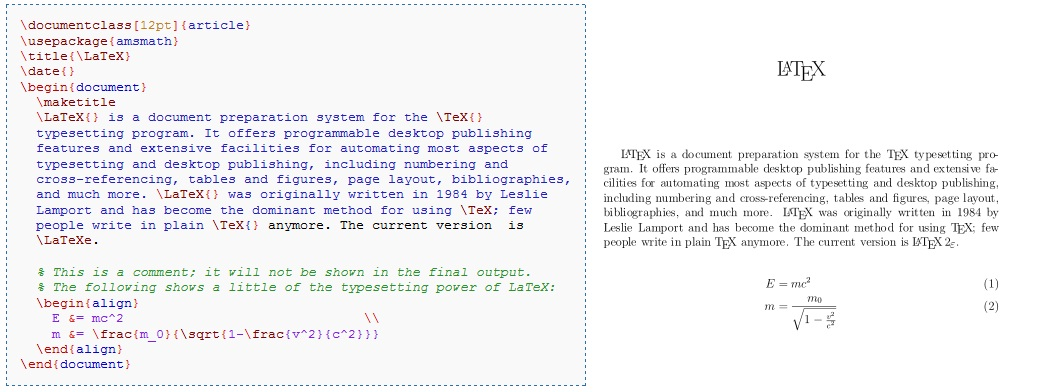
\includegraphics[width=1\textwidth]{prestudy/latex.JPG}
	\caption{LaTeX input and corresponding output}
	\label{fig:latex}
\end{figure}

LaTeX is based on the idea that authors should be able to focus on the content of what they are writing without being distracted by its visual presentation. In preparing a LaTeX document, the author specifies the logical structure using familiar concepts such as chapter, section, table, figure, etc., and lets the LaTeX system worry about the presentation of these structures. It therefore encourages the separation of layout from content while still allowing manual typesetting adjustments where needed. This is similar to the mechanism by which many word processors allow styles to be defined globally for an entire document or the use of Cascading Style Sheets to style HTML.\newline

LaTeX can be arbitrarily extended by using the underlying macro language to develop custom formats. Such macros are often collected into packages, which are available to address special formatting issues such as complicated mathematical content or graphics. Indeed, in the example below, the align environment is provided by the amsmath package.